\documentclass{beamer}

\usepackage[utf8]{inputenc}
\usepackage{minted}
\usepackage{listings}
\usepackage{graphicx}



%\usetheme{Warsaw}
\usetheme{metropolis}
\usecolortheme{beaver}

\title[Kubernetes]{Introduction to Kubernetes}
\author{Ed MacDonald}
\institute{Solution Street}
\date{June 2020}

\begin{document}
\frame{\titlepage}

\begin{frame}
\frametitle{What is Kubernetes?}
A Declarative Container Orchestration Framework
\end{frame}

\begin{frame}
\frametitle{Declarative}
Most Kubernetes API calls involve either:
\begin{itemize}
    \item You telling Kubernetes what you want the state of a given set of objects to converge to, or
    \item You asking Kubernetes what the current state of a given set of objects currently is
\end{itemize}
\end{frame}

\begin{frame}
\frametitle{Container}
The fundamental building blocks of an application deployed on Kubernetes are Containers.
\end{frame}

\begin{frame}
\frametitle{Orchestration}
Once you declare to Kubernetes what you want the state of a cluster to be, Kubernetes works to make it so, by doing things like:
\begin{itemize}
    \item Ensuring the desired number of containers are running by starting new ones when existing ones crash.
    \item Load balancing traffic between running containers based on you declaring your wish for it to do so.
    \item Starting/Stopping Pods during times of heavy/light resource utilization.
\end{itemize}
\end{frame}

\begin{frame}
\frametitle{Kubernetes API}
\begin{itemize}
    \item Think of the Kubernetes API as a way to send and receive Kubernetes objects to and from the Kubernetes Control Plane.
    \item Objects are represented as structured documents. We'll use Yaml, but I bet with some work you could use JSON or even XML.
\end{itemize}
\end{frame}

\begin{frame}
\frametitle{I Lied. Lets talk about Pods.}
I said Containers were the fundamental building blocks. Technically, Pods are. What's a Pod?
\begin{itemize}
    \item A Pod is a group of one or more containers that work closely together on a specific task.
    \item Containers in a Pod can share the same volume mounts.
    \item Some Containers in a Pod can be Init Containers. They run before other pods start and are used to perform startup work. The can communicate with other pods through the aforementioned shared volumes.
\end{itemize}
\end{frame}

\begin{frame}
\frametitle{ReplicaSets}
\begin{itemize}    
    \item ReplicaSets allow you to declare to Kubernetes how many of a given type of Pod you wish to have running.
    \item Pods in a ReplicaSet are treated as if they are Stateless.
\end{itemize}
\end{frame}


\begin{frame}
\frametitle{Summary of Tools Used}
\begin{itemize}
    \item This is a text in the first frame. This is a text in the first frame. This is a text in the first frame. How long until it updates in the preview?
\end{itemize}
\end{frame}

\begin{frame}
More frames
\end{frame}

\begin{frame}
\frametitle{Tools used}
\begin{itemize}
    \item Minikube (https://kubernetes.io/docs/tasks/tools/install-minikube/)
(will also have you install a hypervisor (eg: VirtualBox) and kubectl)
    \item Helm (https://helm.sh/docs/intro/install/)
\end{itemize}
\end{frame}

\begin{frame}
\frametitle{Other Resources}
\begin{itemize}
    \item http://files.pushshift.io/reddit/subreddits/
\end{itemize}
\end{frame}

\begin{frame}
\frametitle{What’s Still To Do?}
\begin{block}{Answered Questions}
    How many primes are there?
\end{block}
\begin{block}{Open Questions}
    Is every even number the sum of two primes?
\end{block}
\end{frame}

\begin{frame}
\frametitle{What’s Still To Do?}
\begin{columns}
    \column{.25\textwidth}
    \begin{block}{Answered Questions}
        How many primes are there?
    \end{block}
    \column{.75\textwidth}
    \begin{block}{Open Questions}
        Is every even number the sum of two primes?
    \end{block}
\end{columns}
\end{frame}

\begin{frame}[fragile]
\frametitle{An Algorithm For Finding Prime Numbers.}
\begin{minted}{cpp}
int main (void)
{
    std::vector<bool> is_prime (100, true);
    for (int i = 2; i < 100; i++)
        if (is_prime[i])
        {
            std::cout << i << " ";
            for (int j = i; j < 100; is_prime [j] = false, j+=i);
        }
    return 0;
}
\end{minted}
\end{frame}

\begin{frame}[fragile]
\frametitle{Yaml?}
\begin{columns}
    \column{.25\textwidth}
    \begin{block}{Answered Questions}
        How many primes are there?
    \end{block}
    \column{.75\textwidth}
    \begin{block}{Open Questions}
\begin{minted}[style=friendly,fontsize=\fontsize{3}{4}]{yaml}
---
apiVersion: v1
kind: Pod
metadata:
  namespace: default
  name: demo-demo-6f95ccf6d5-pdnmc
  labels:
    app.kubernetes.io/instance: demo
    app.kubernetes.io/name: demo
spec:
  containers:
  - image: nginx:1.16.0
    name: demo
    livenessProbe:
      httpGet:
        path: /
        port: http
        scheme: HTTP
    ports:
    - containerPort: 80
      name: http
      protocol: TCP
    readinessProbe:
      httpGet:
        path: /
        port: http
        scheme: HTTP
    volumeMounts:
    - mountPath: /var/run/secrets/kubernetes.io/serviceaccount
      name: demo-demo-token-dj7lr
      readOnly: true
  volumes:
  - name: demo-demo-token-dj7lr
    secret:
      defaultMode: 420
      secretName: demo-demo-token-dj7lr

\end{minted}
    \end{block}
\end{columns}
\end{frame}

% https://www.patrickbaylis.com/posts/2018-10-11-beamer-resizing/
\begin{frame}
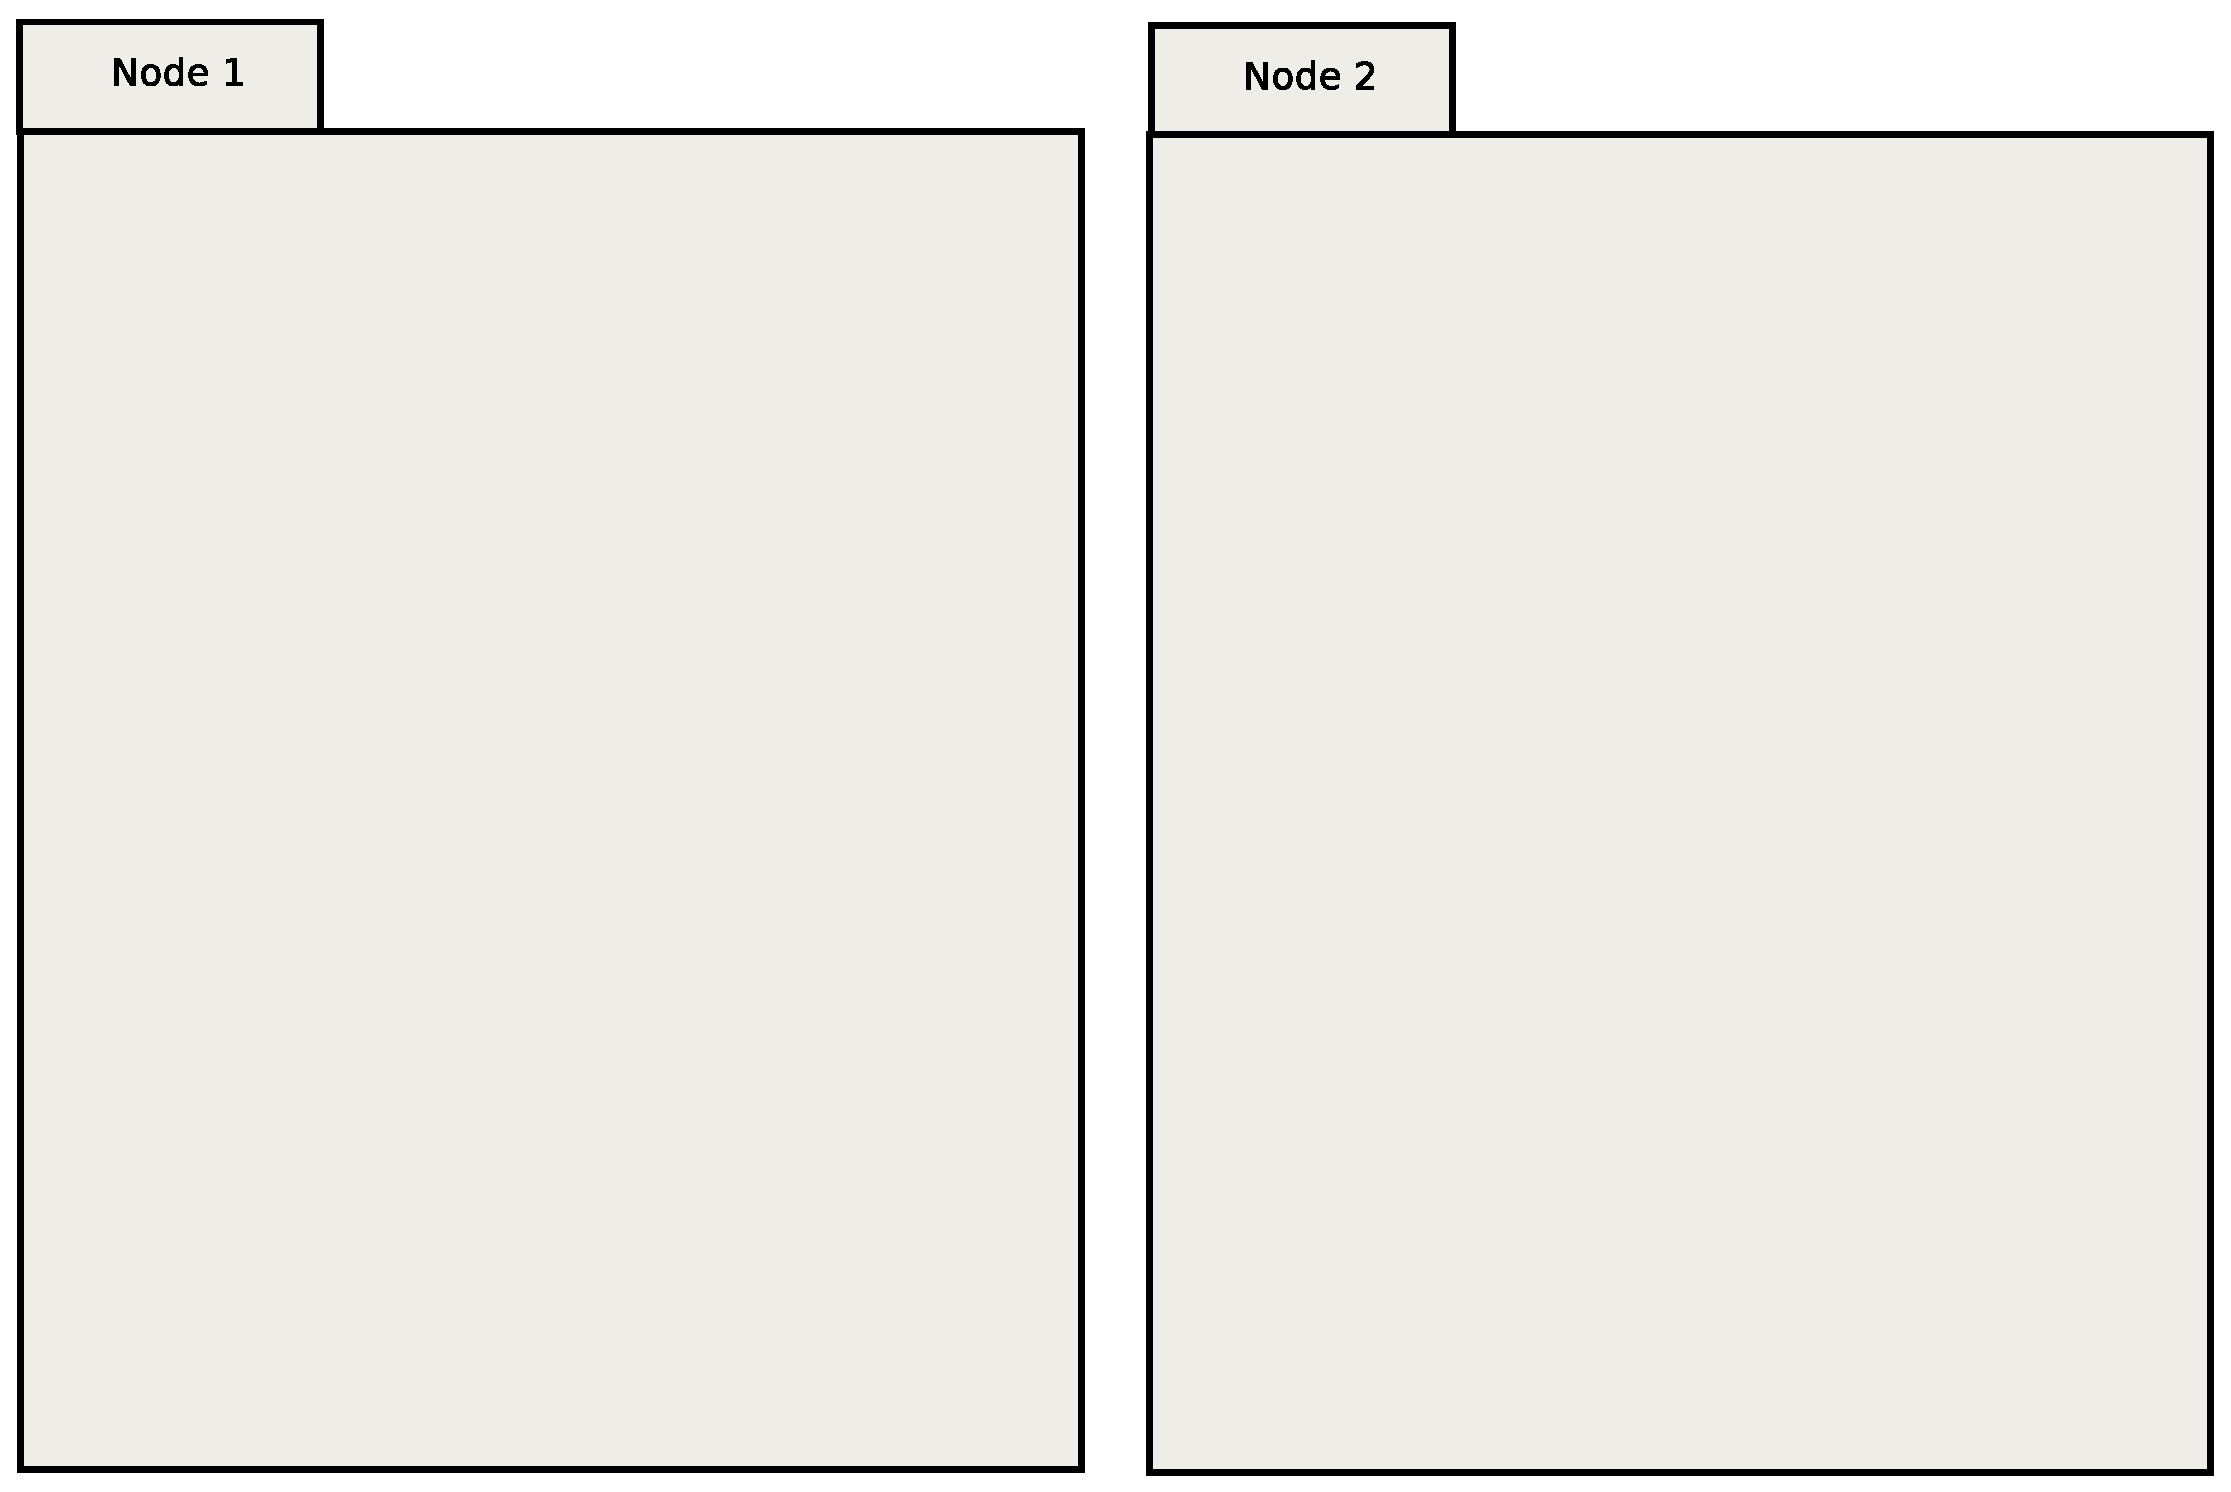
\includegraphics[width=\textwidth,height=\textheight,keepaspectratio]{graphics/00-nodes.eps}
\end{frame}

\begin{frame}
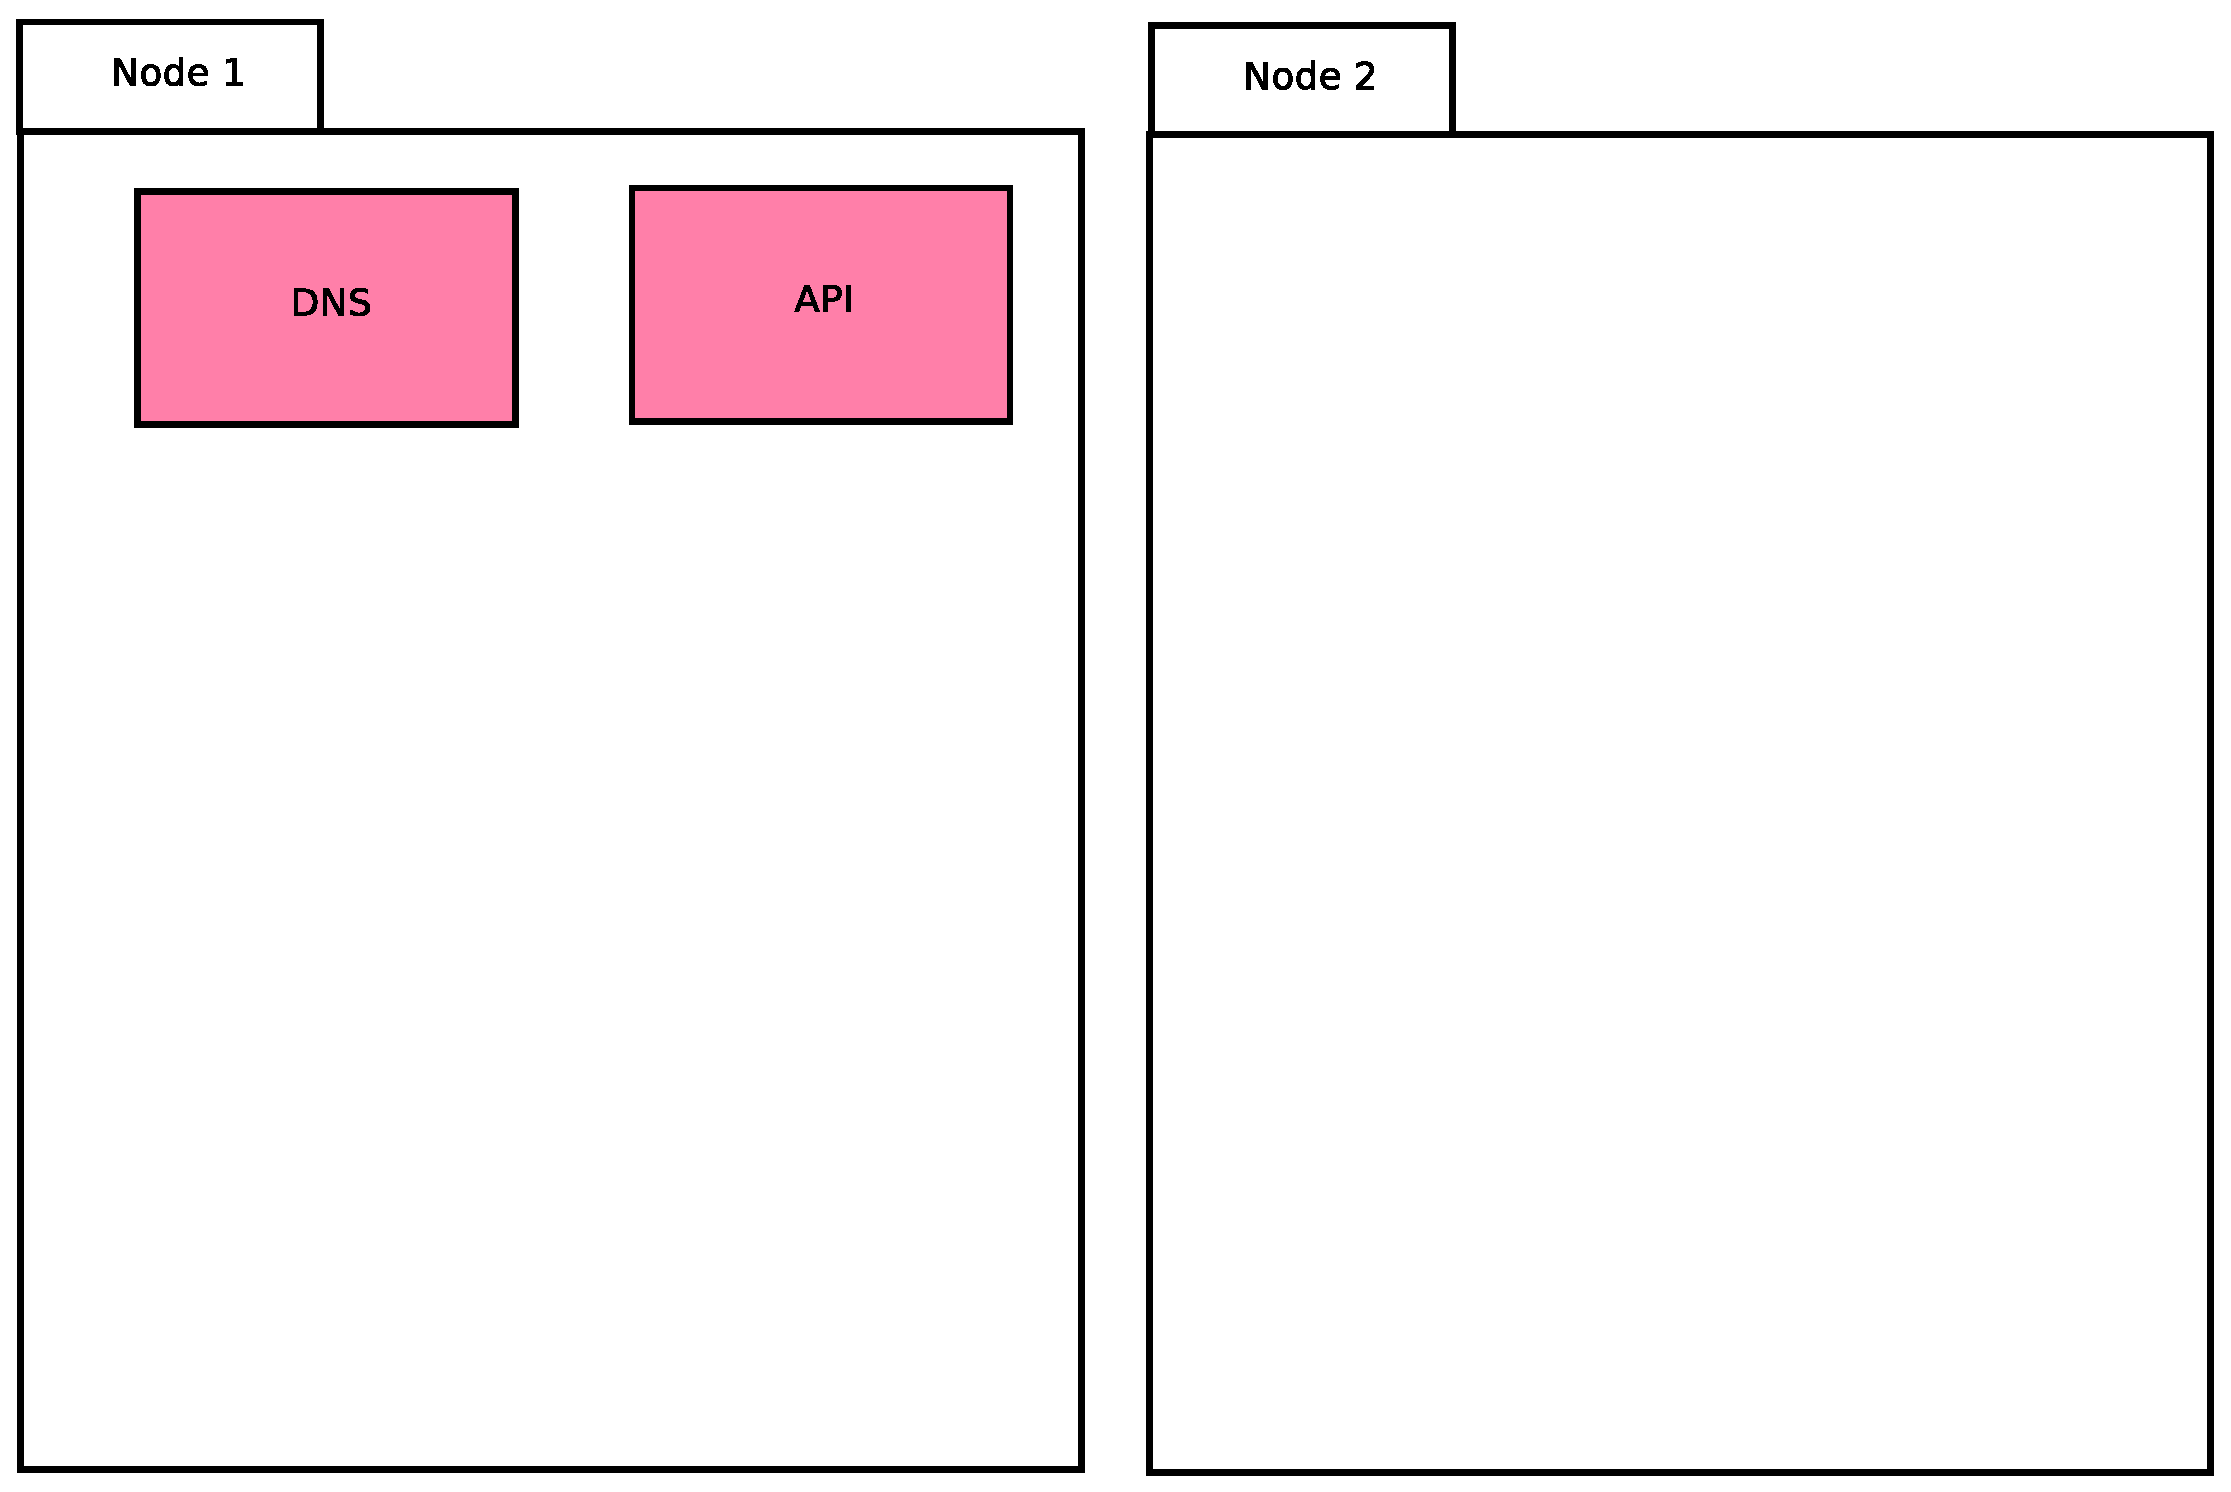
\includegraphics[width=\textwidth,height=\textheight,keepaspectratio]{graphics/01-systemPods.eps}
\end{frame}

\begin{frame}
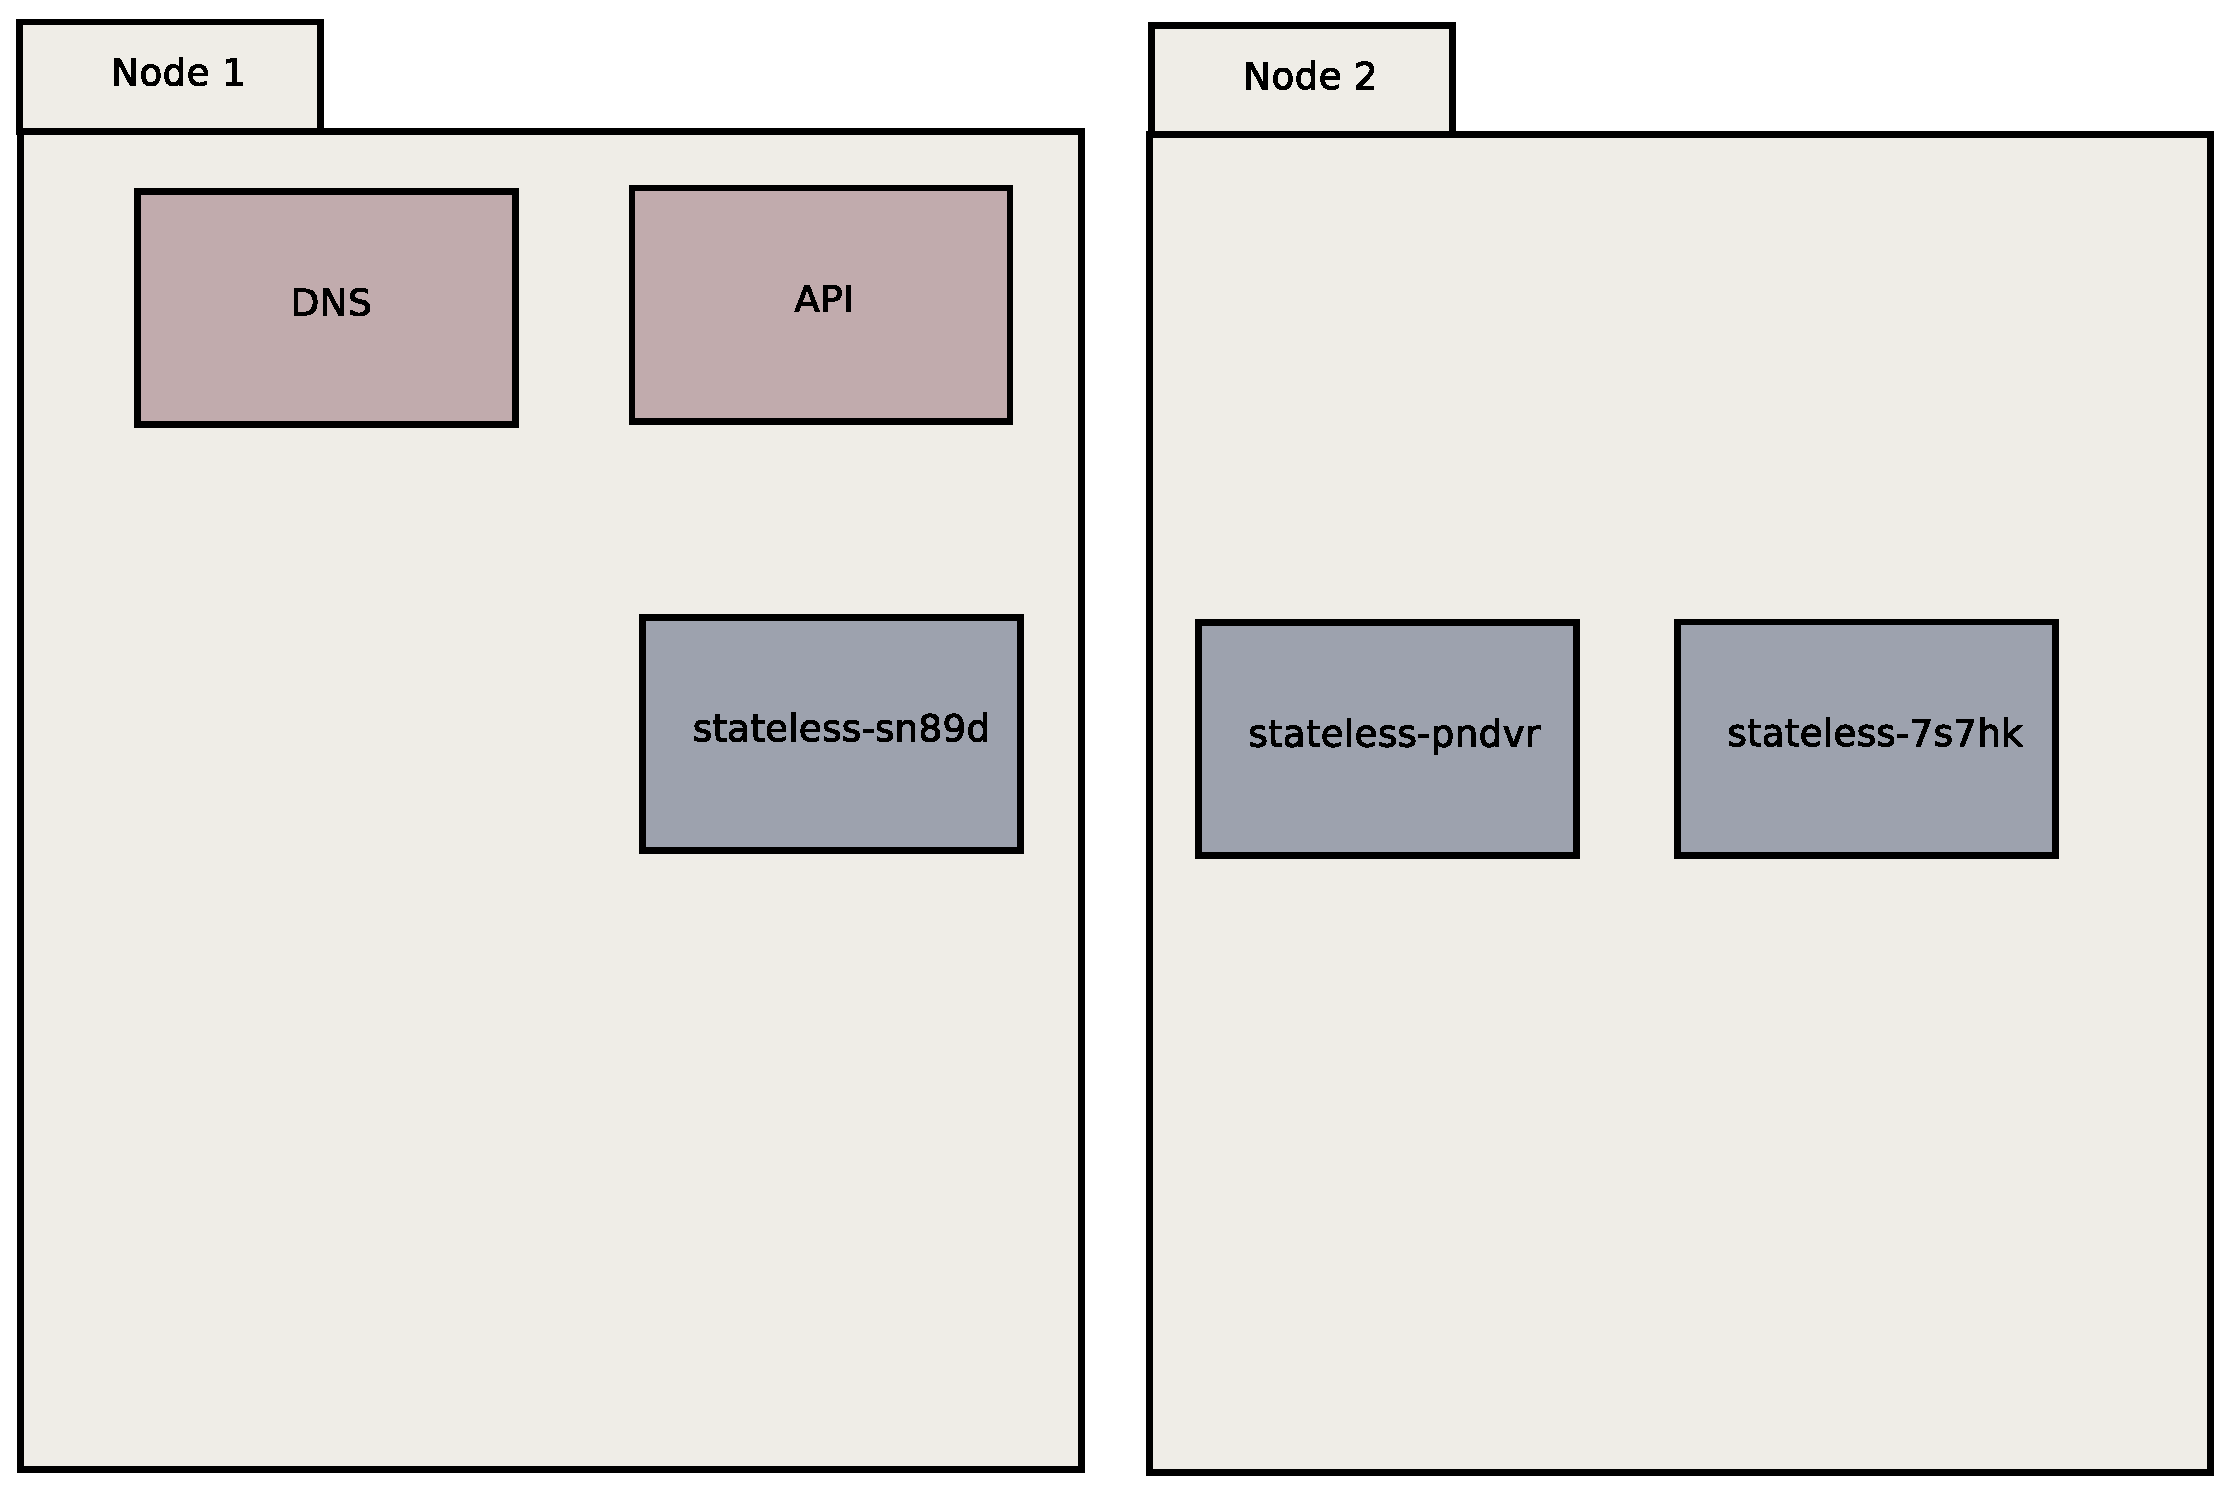
\includegraphics[width=\textwidth,height=\textheight,keepaspectratio]{graphics/02-statelessAppPods.eps}
\end{frame}

\begin{frame}
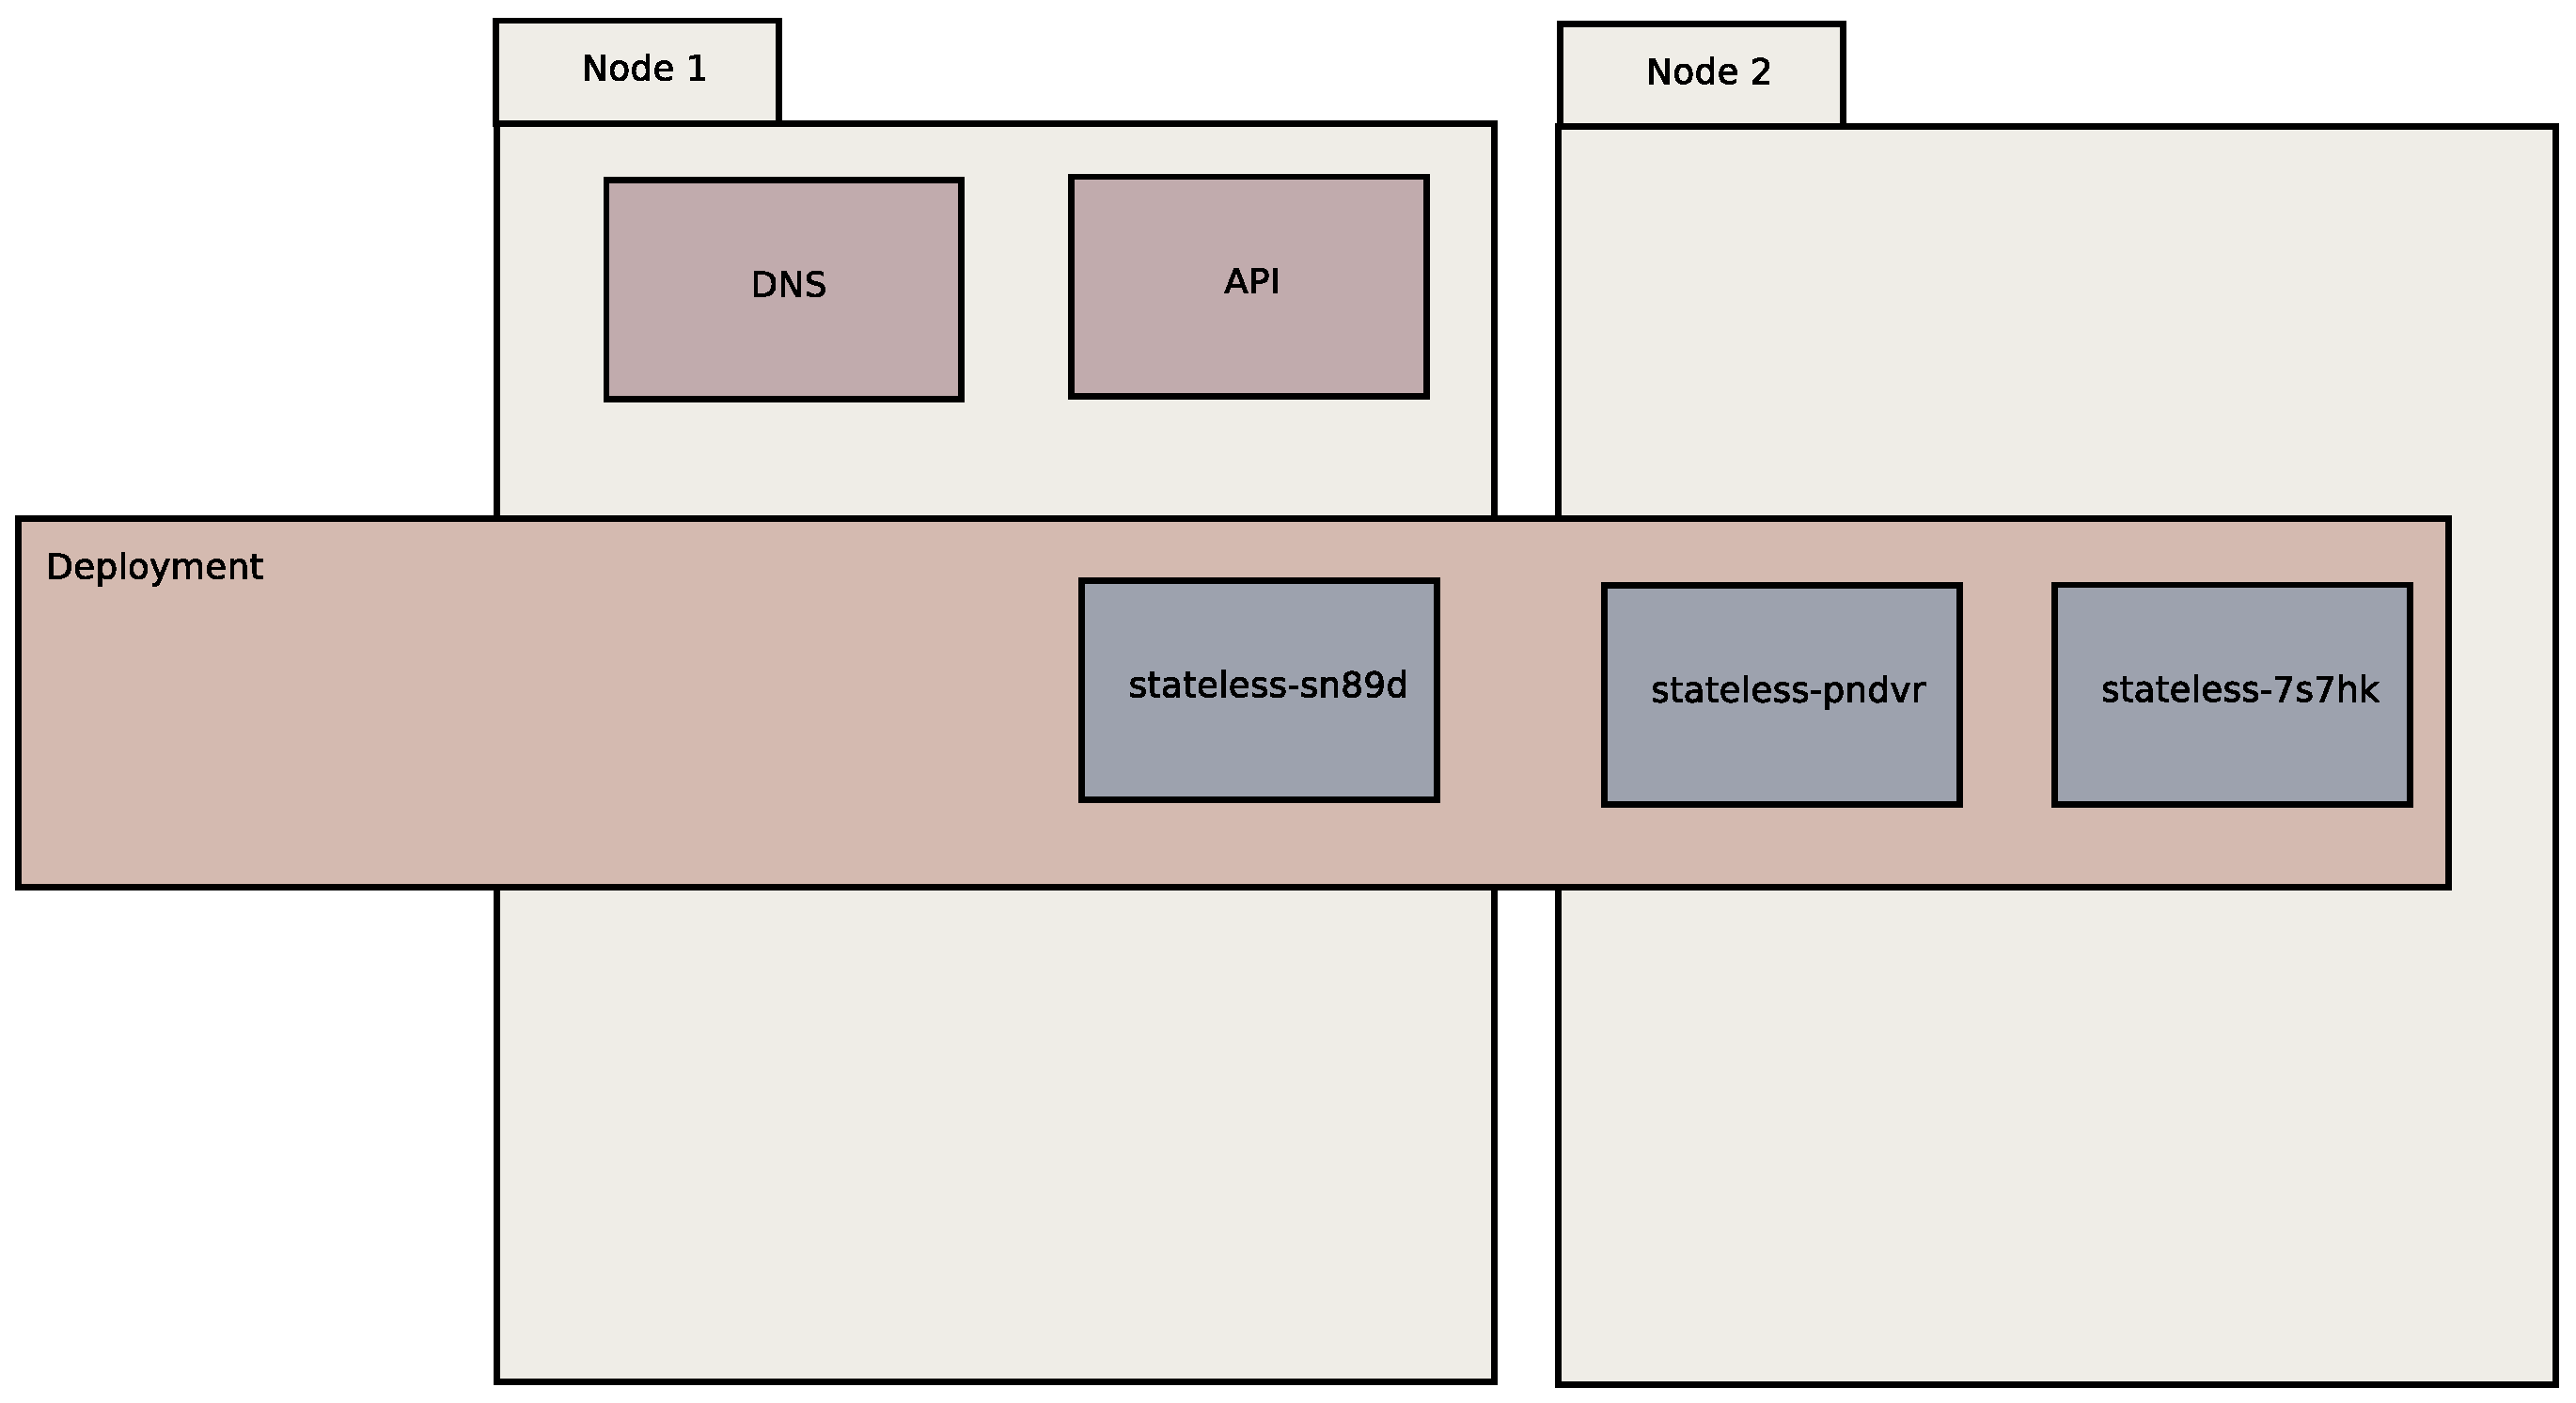
\includegraphics[width=\textwidth,height=\textheight,keepaspectratio]{graphics/03-deployment.eps}
\end{frame}

\begin{frame}
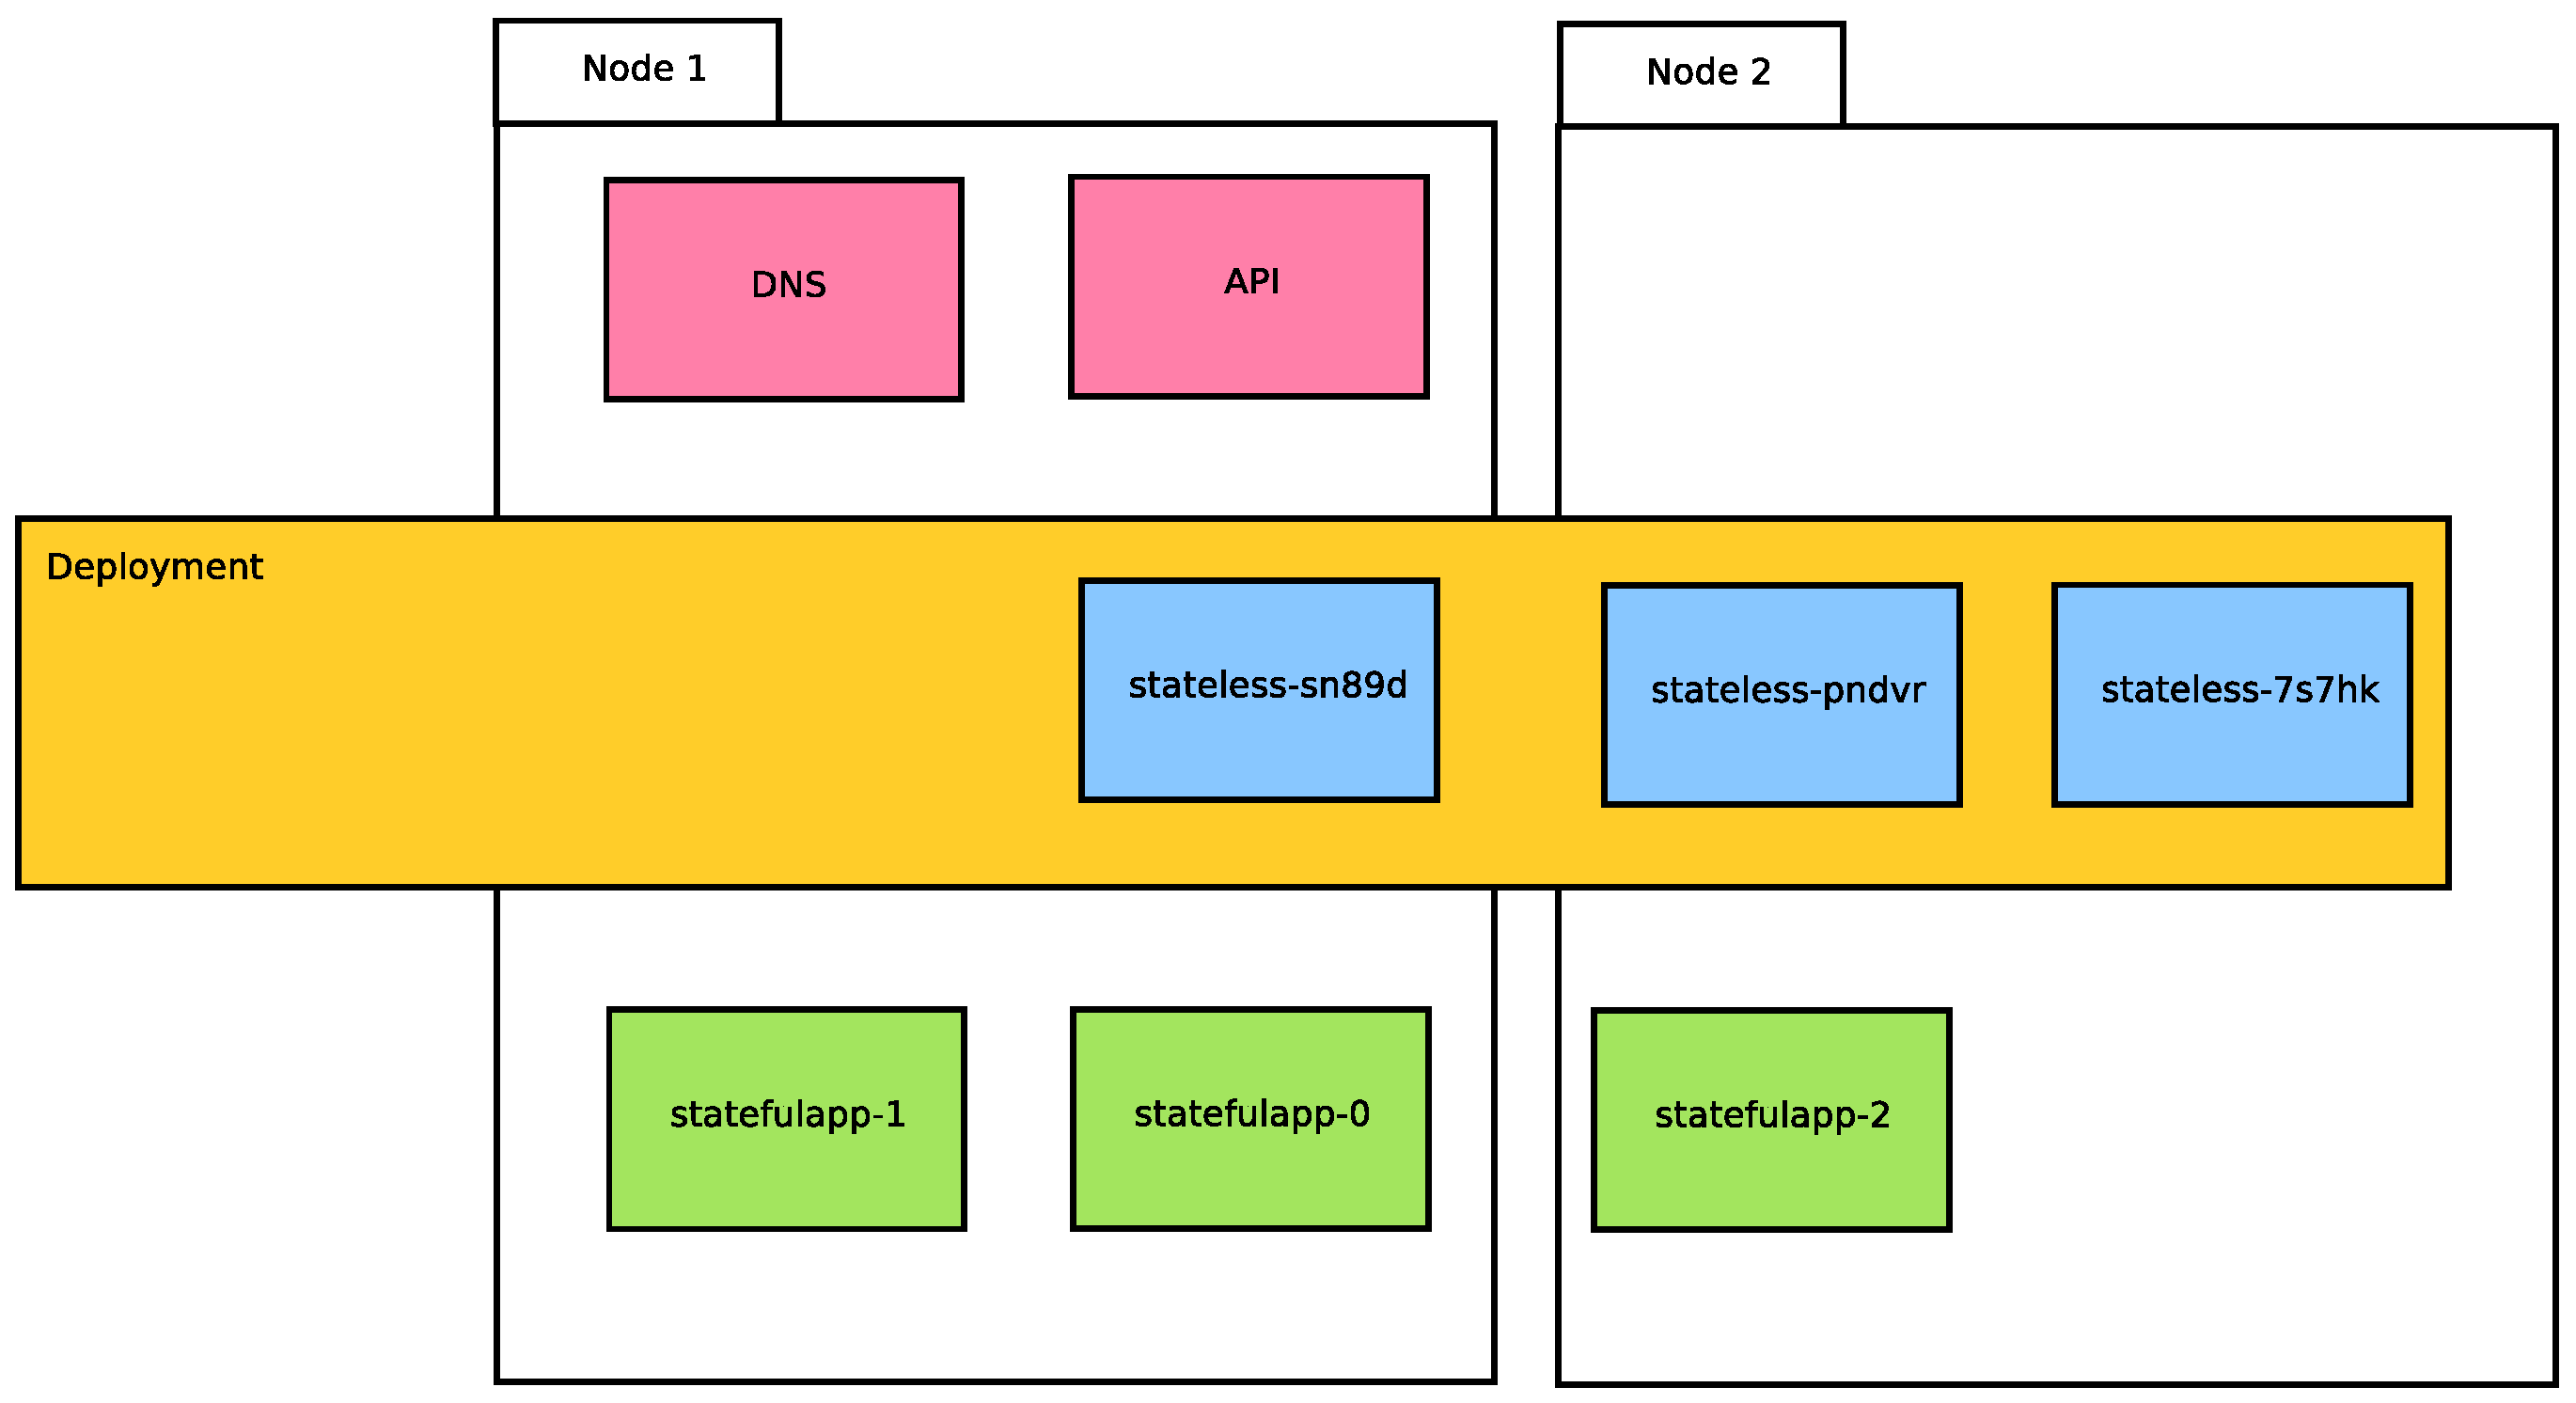
\includegraphics[width=\textwidth,height=\textheight,keepaspectratio]{graphics/04-statefulAppPods.eps}
\end{frame}

\begin{frame}
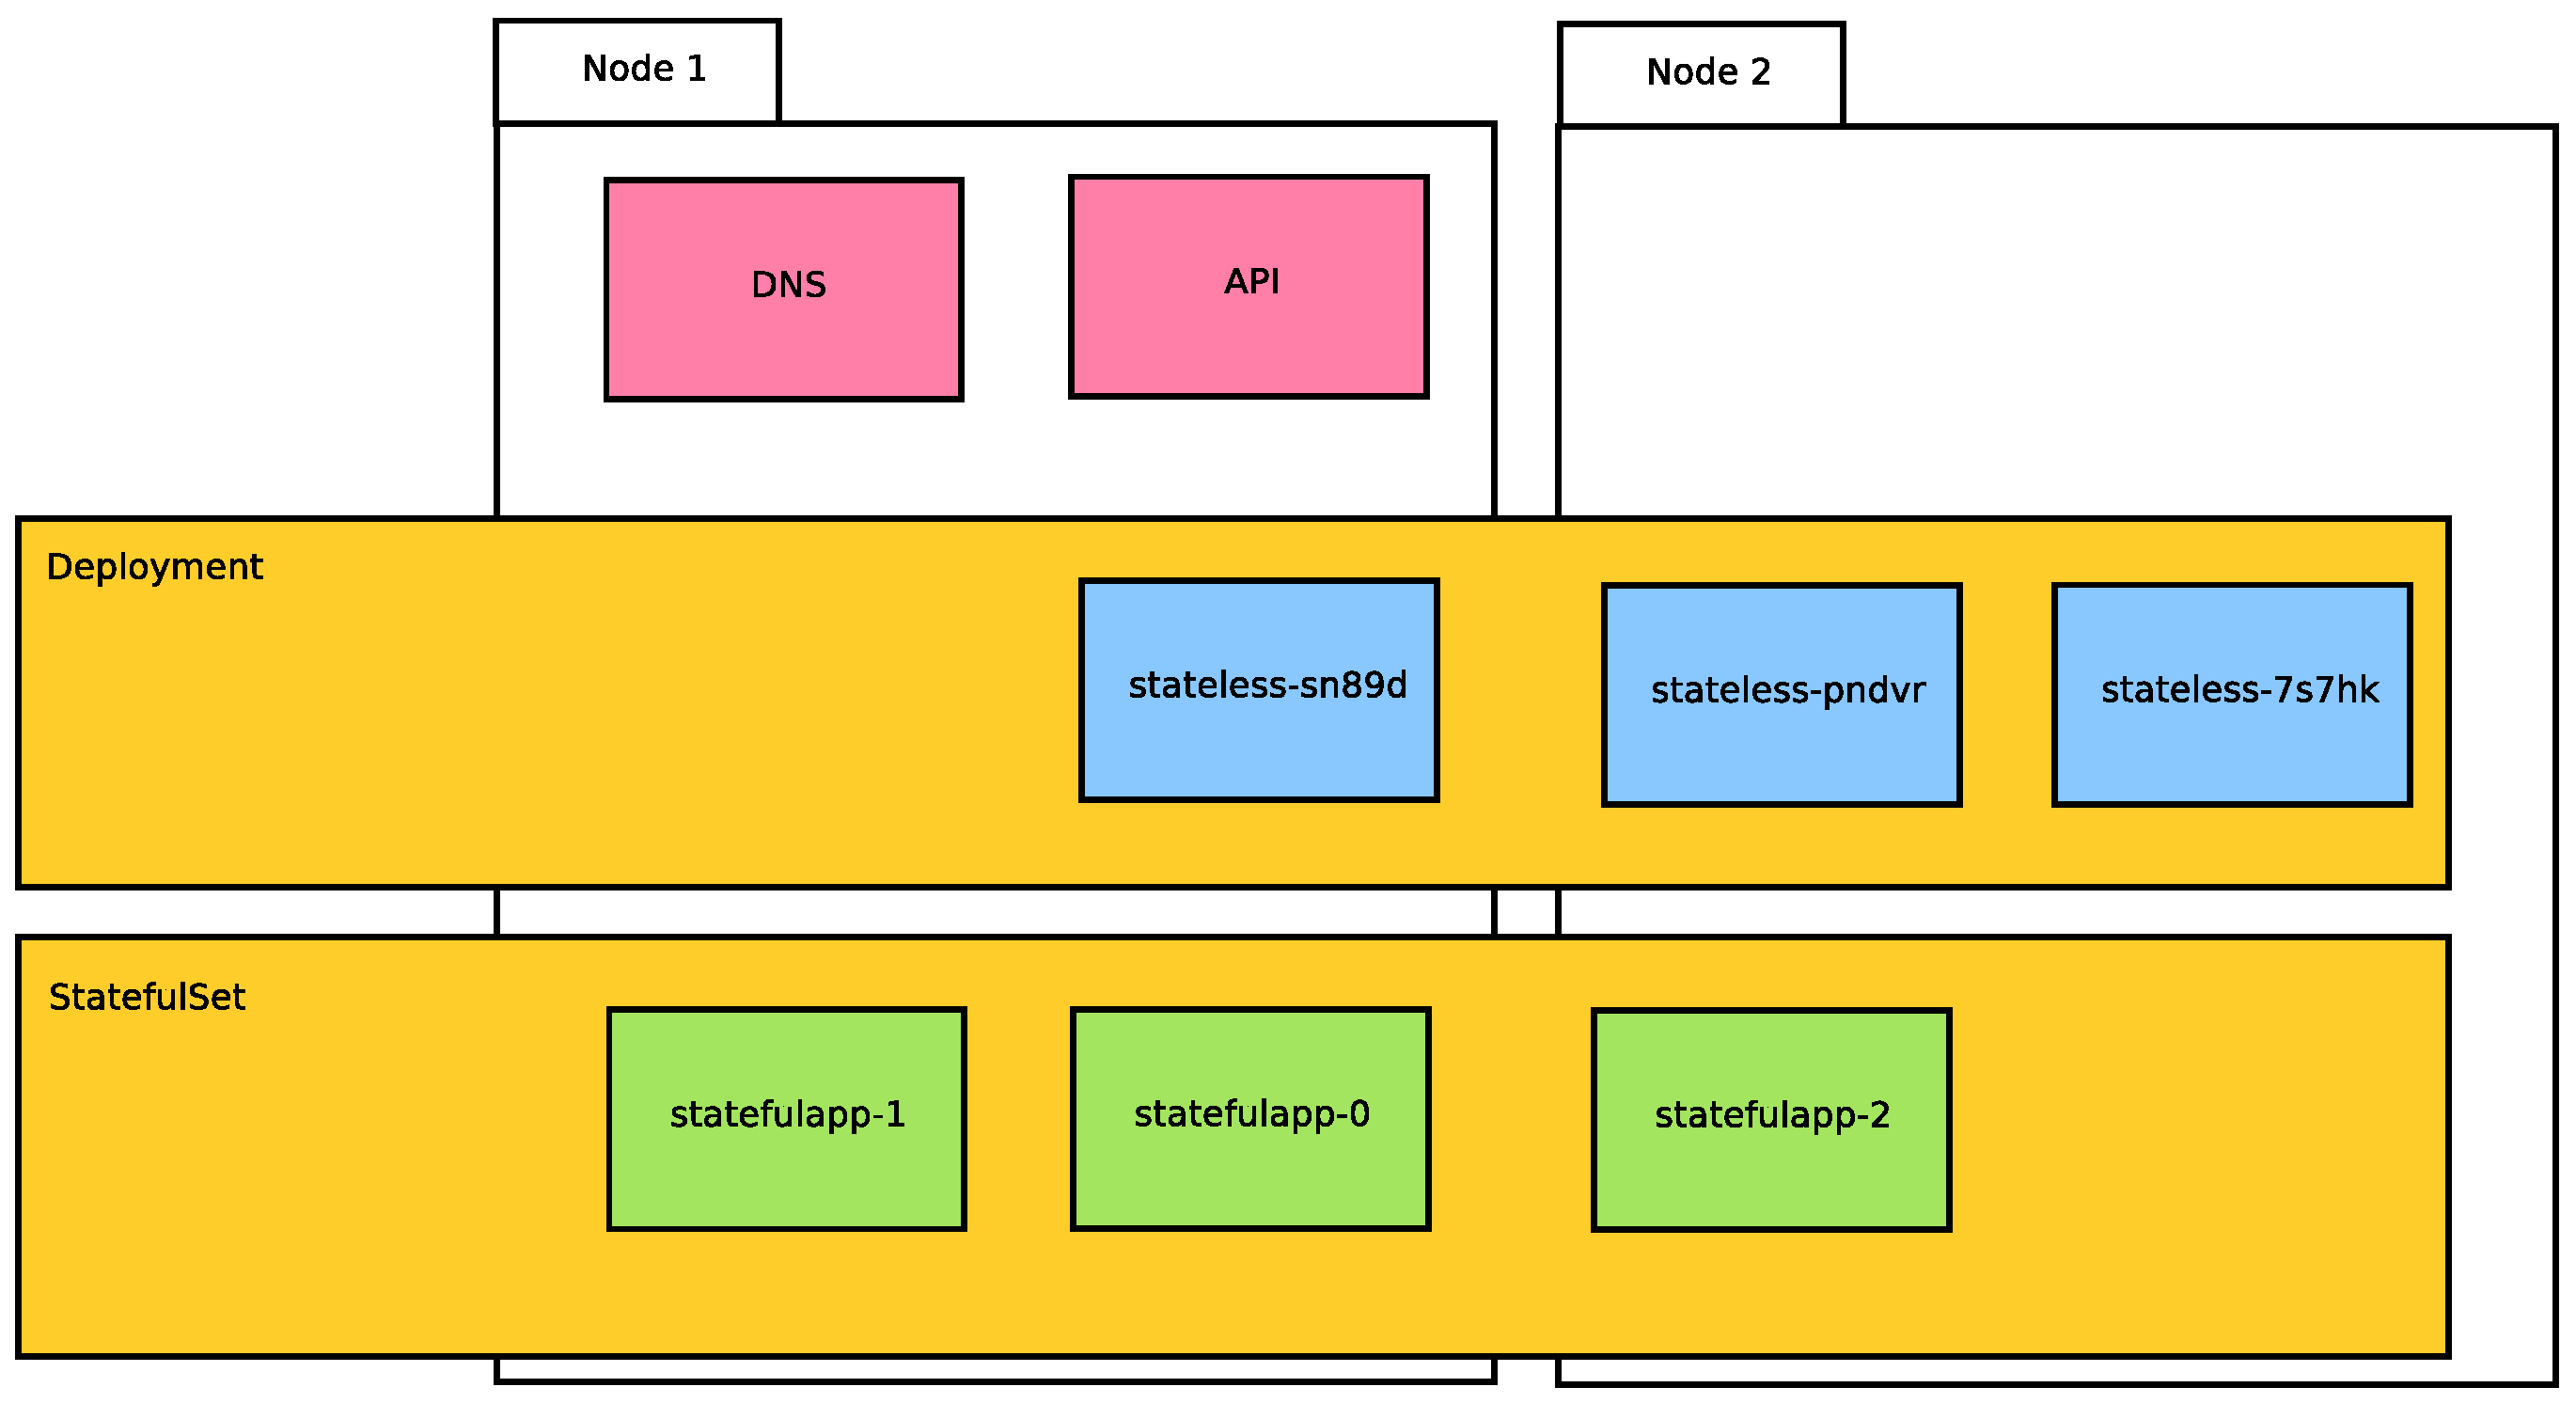
\includegraphics[width=\textwidth,height=\textheight,keepaspectratio]{graphics/05-statefulSet.eps}
\end{frame}

\begin{frame}
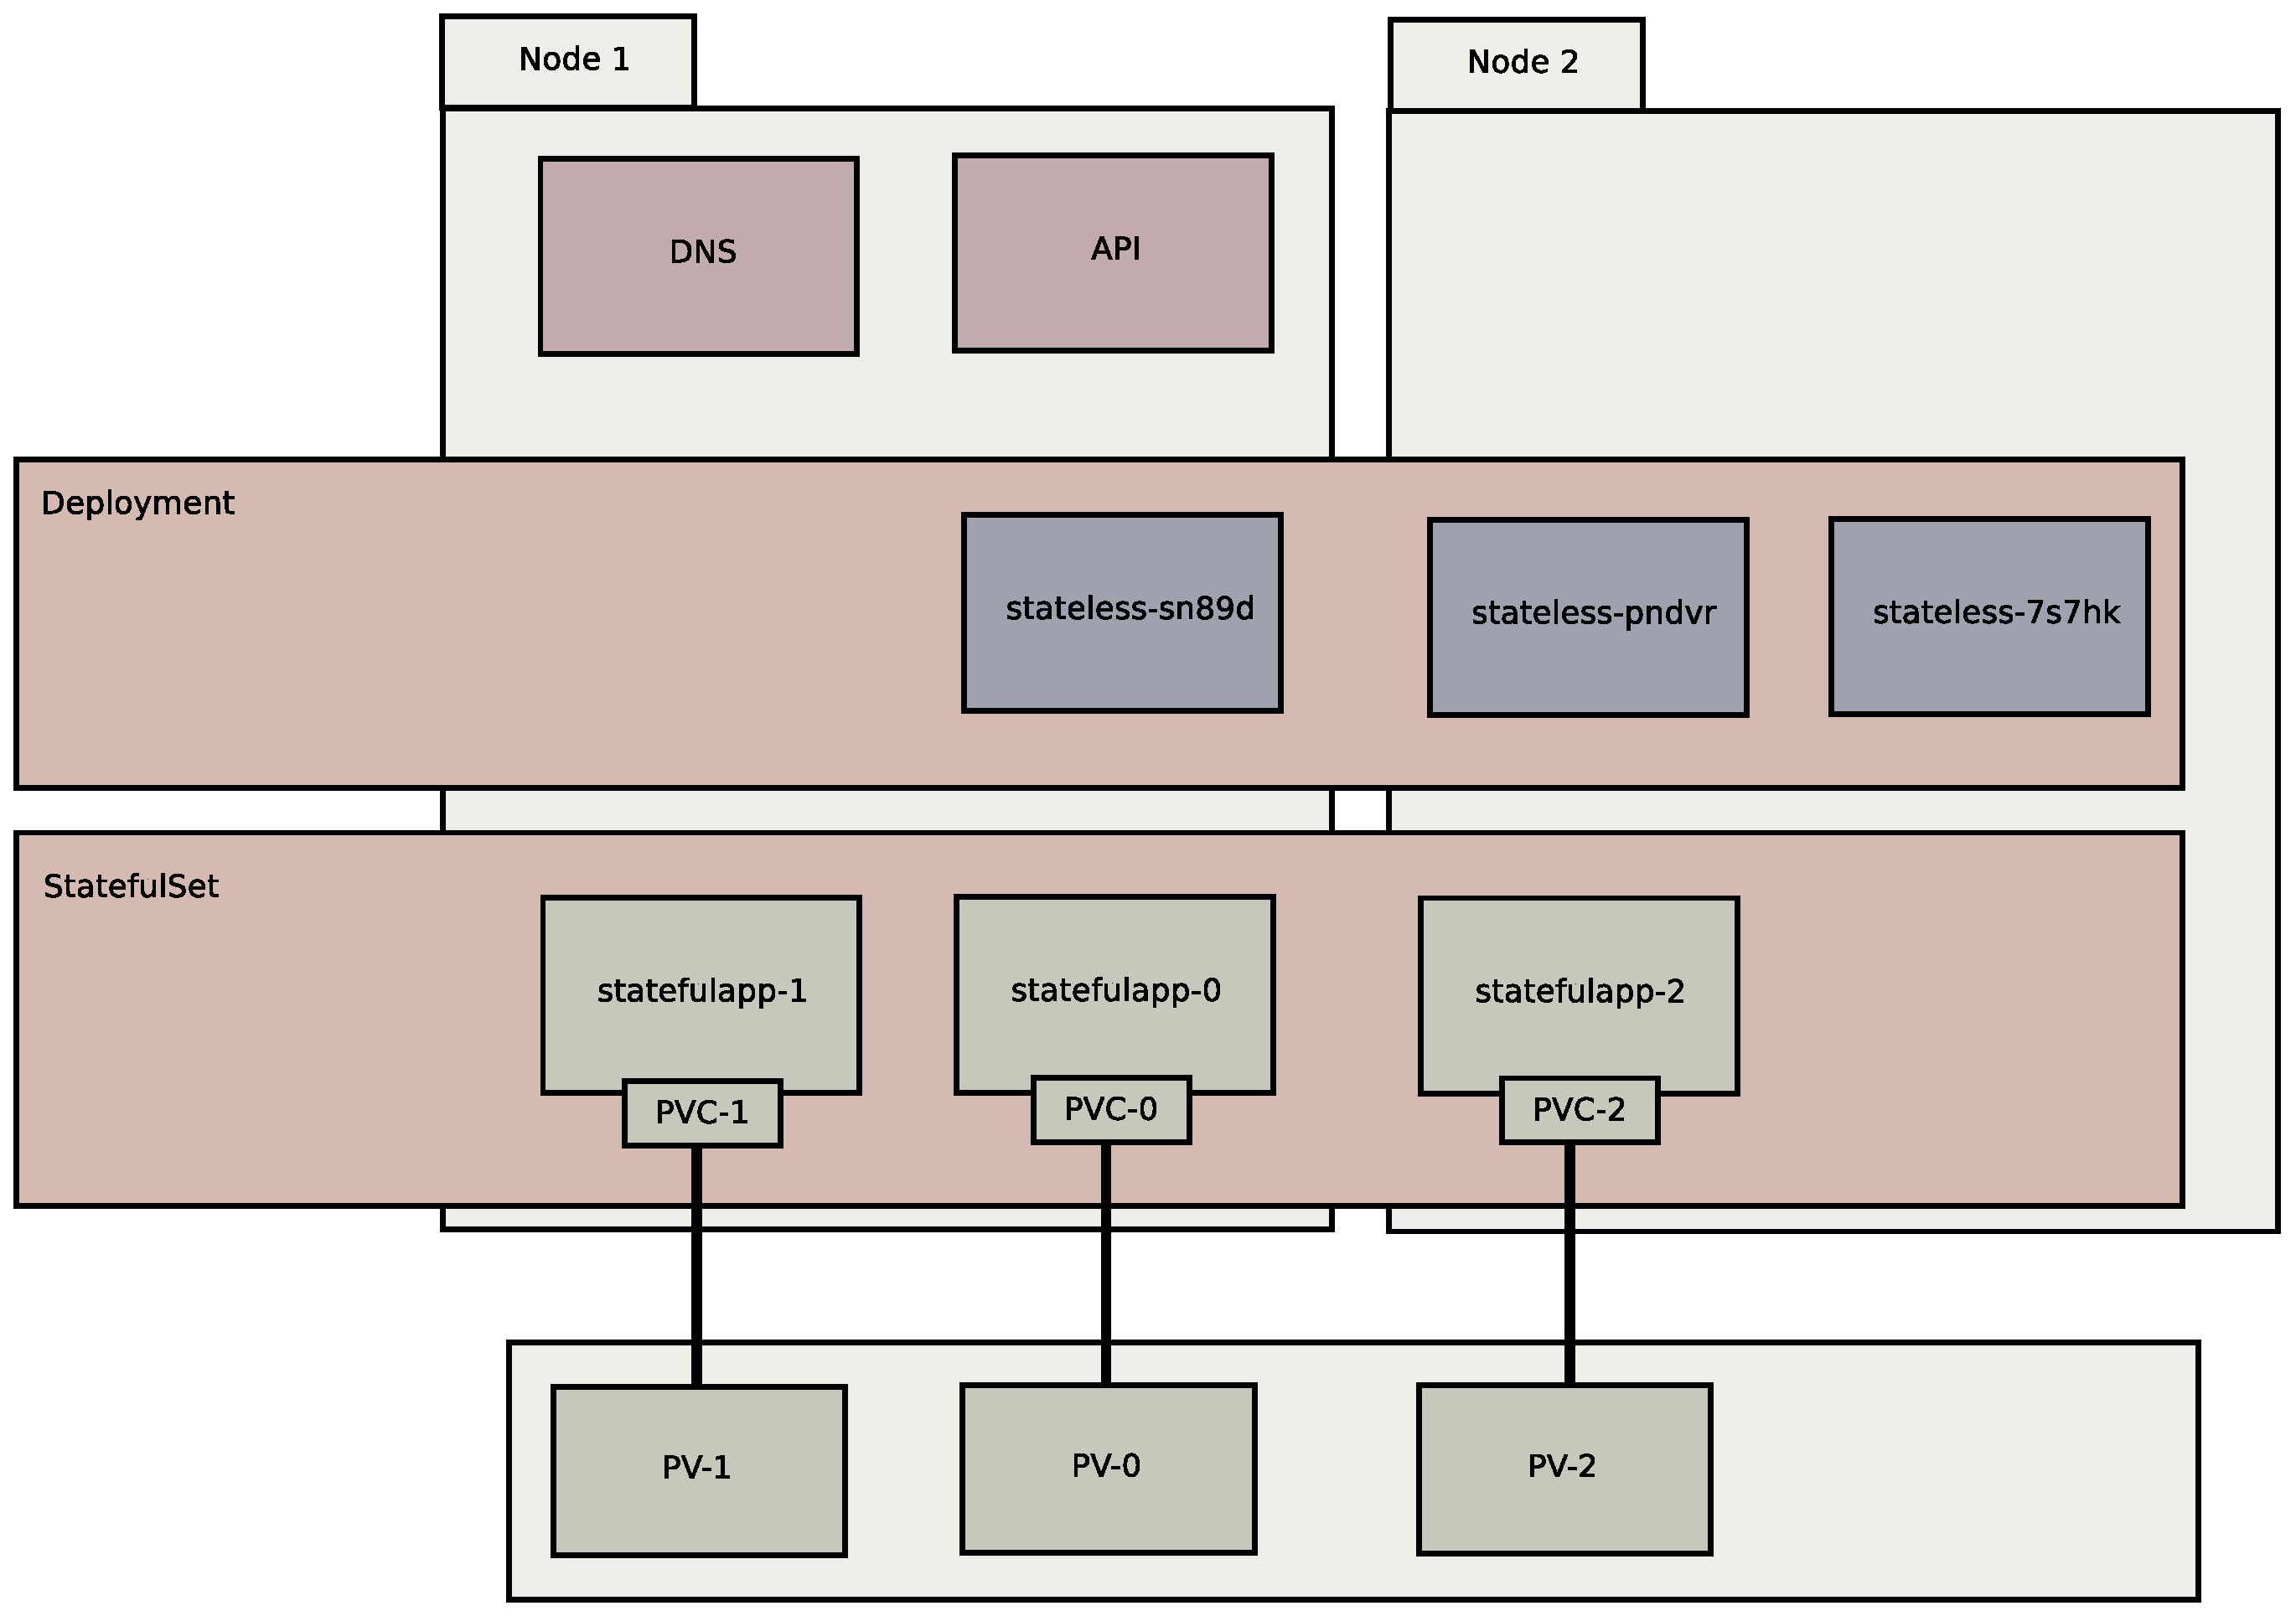
\includegraphics[width=\textwidth,height=\textheight,keepaspectratio]{graphics/06-persistence.eps}
\end{frame}

\begin{frame}
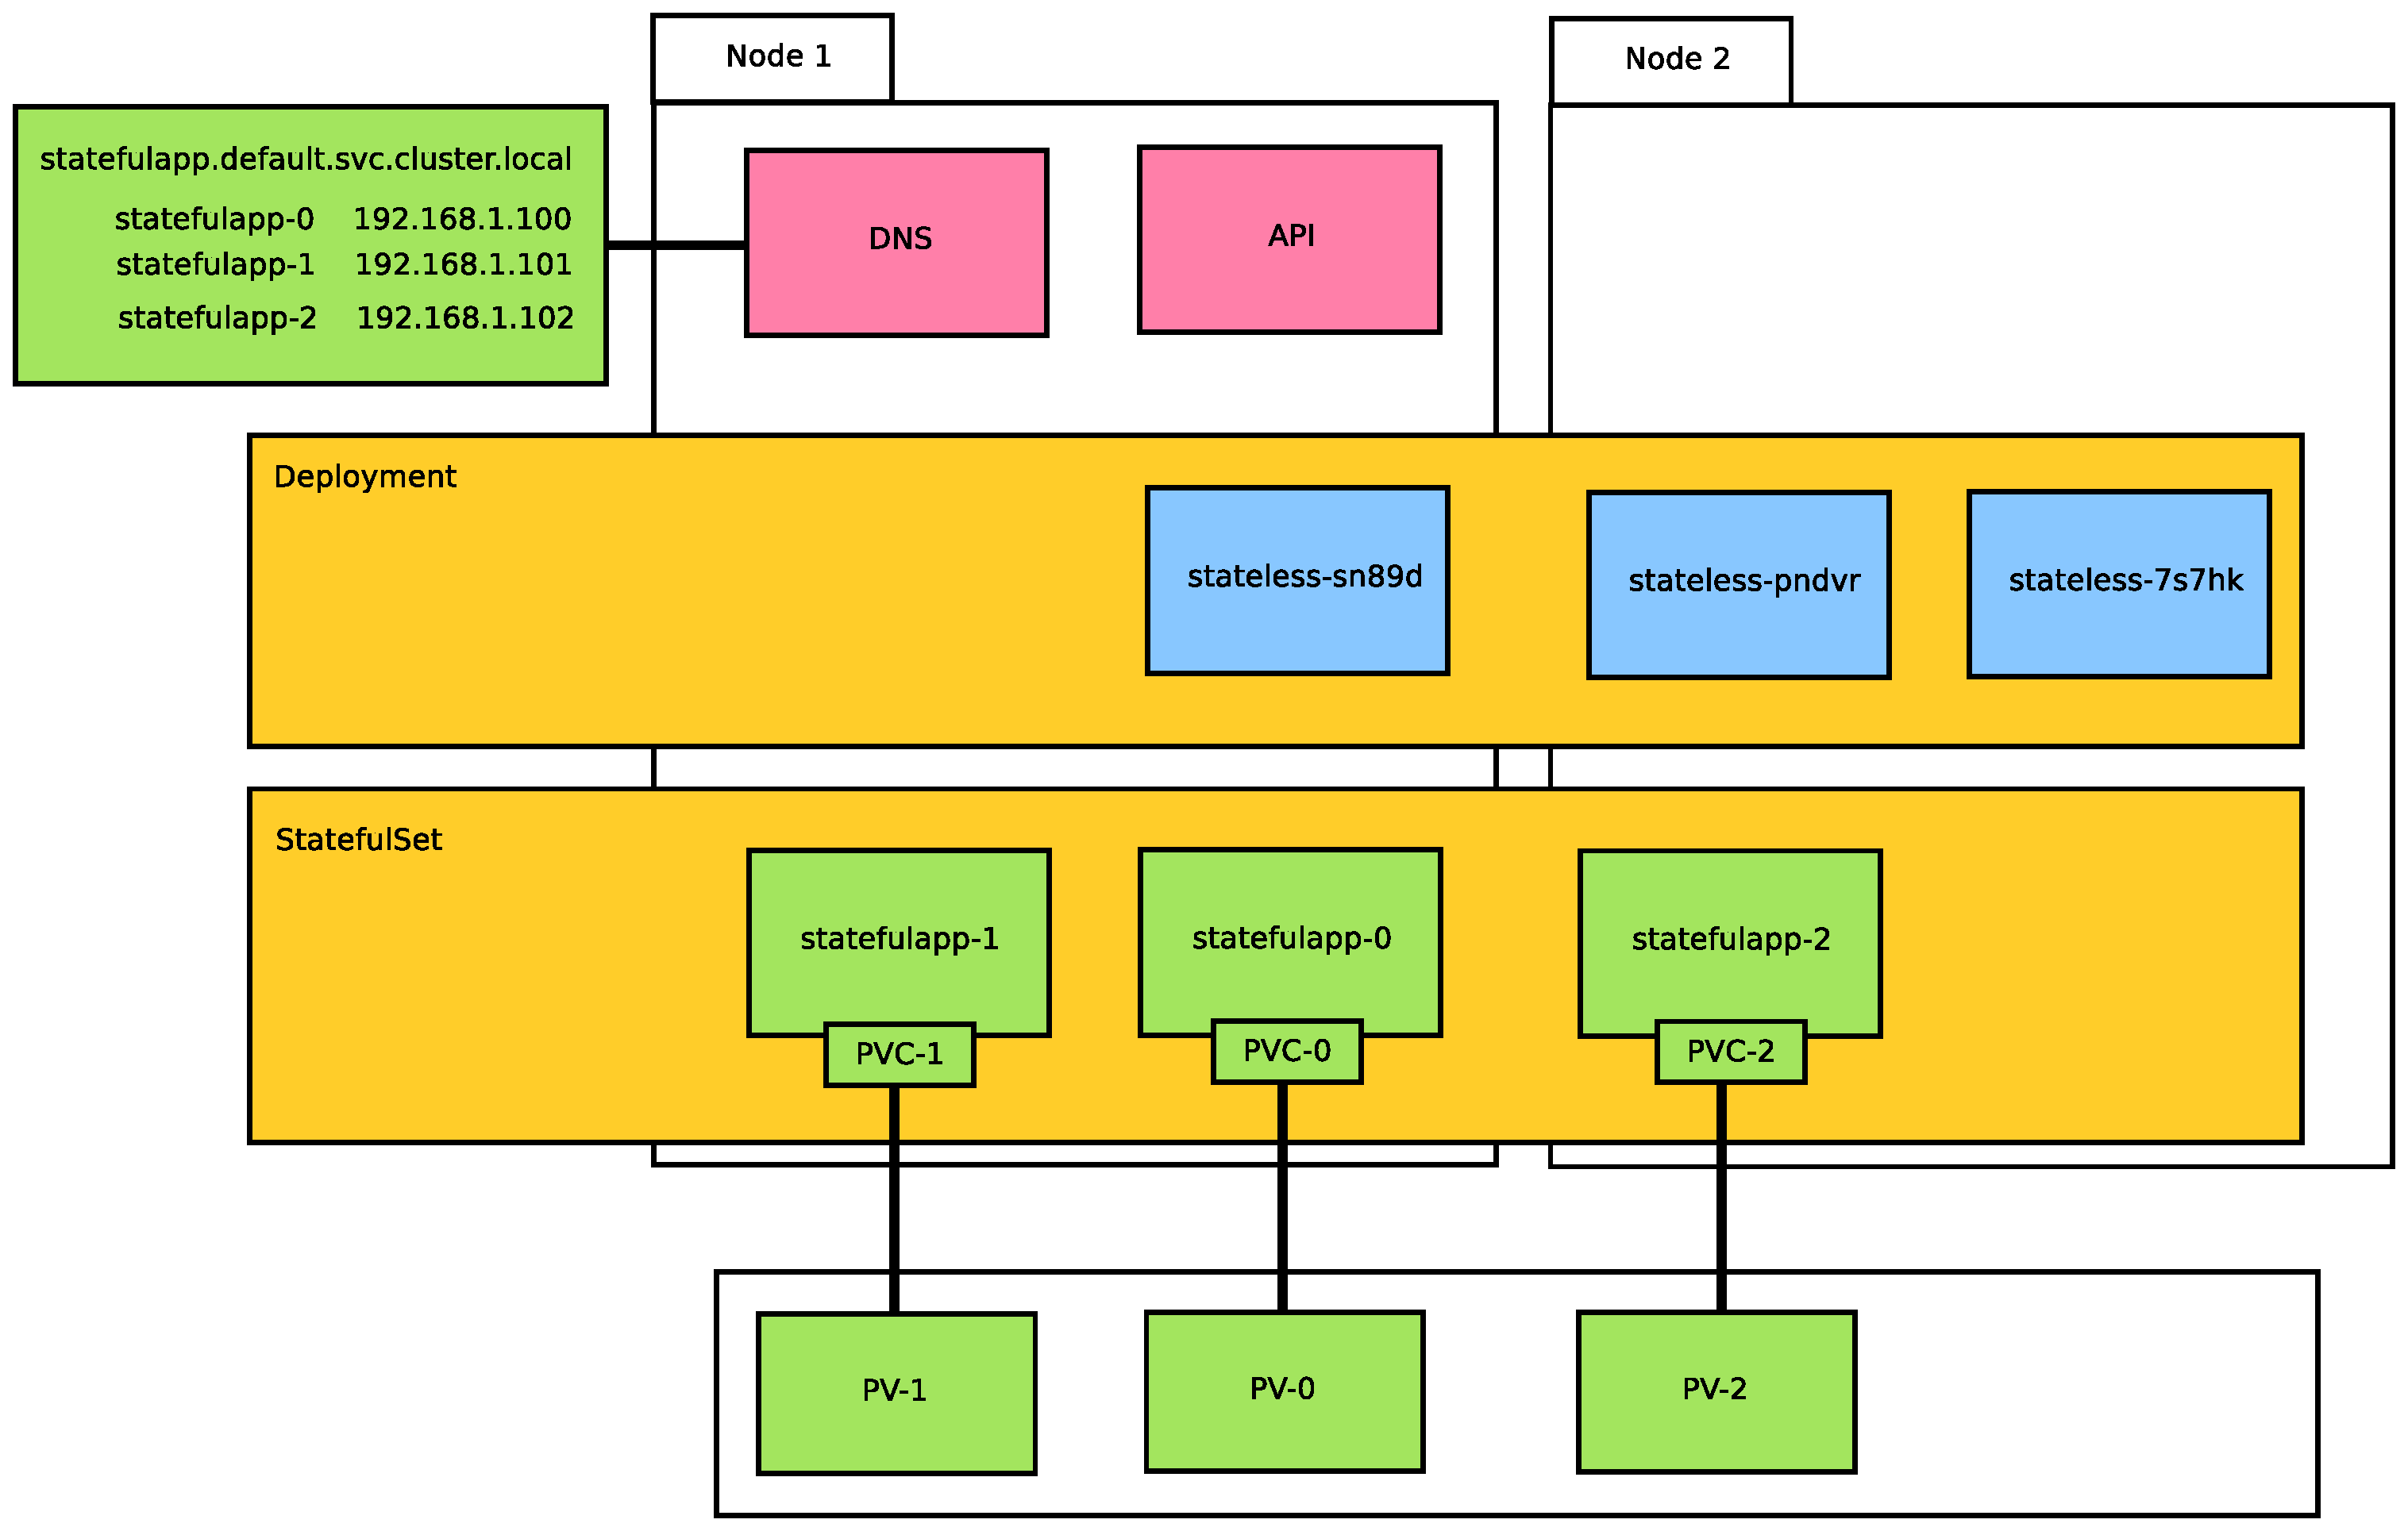
\includegraphics[width=\textwidth,height=\textheight,keepaspectratio]{graphics/07-persistentIdentity.eps}
\end{frame}

\begin{frame}
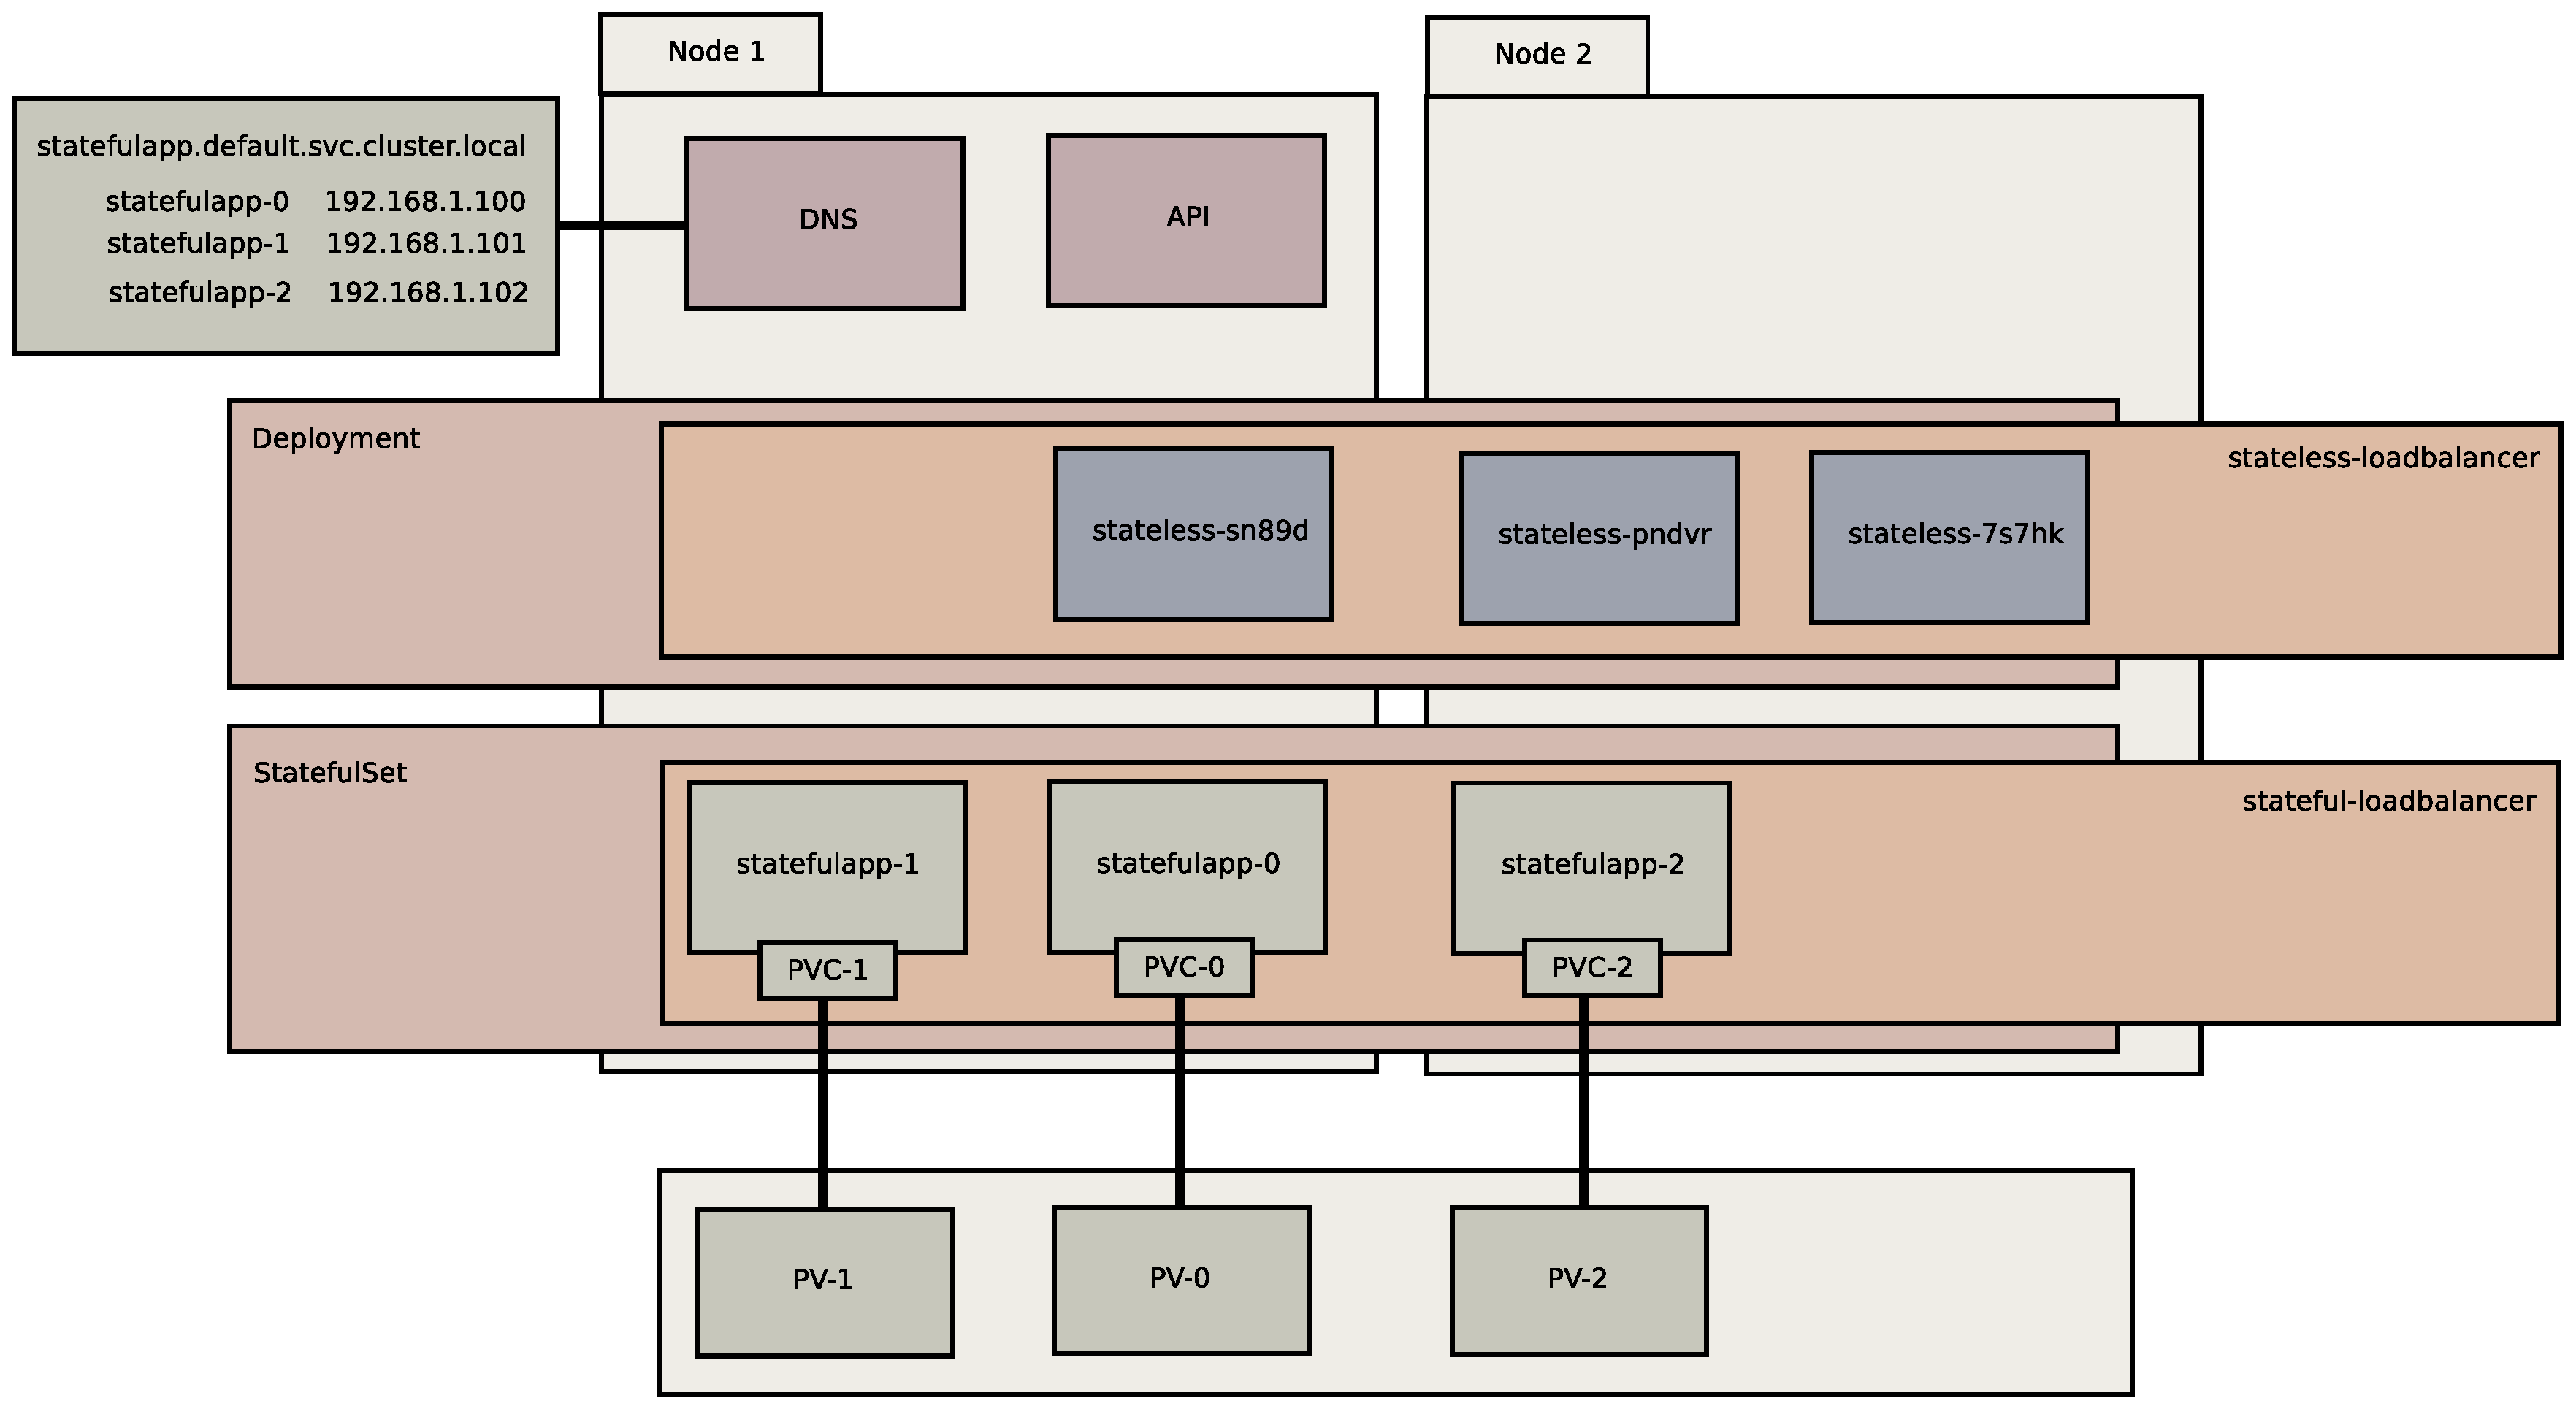
\includegraphics[width=\textwidth,height=\textheight,keepaspectratio]{graphics/08-loadBalancer.eps}
\end{frame}


\end{document}
